\documentclass[../main.tex]{subfiles}

\begin{document}
\subsection{Systematic Reviews}

A systematic review (SR) is one approach, among many, to provide evidence that can be used to support clinical decisions \cite{kranke_evidence-based_2010}. Evidence-based medicine attempts to incorporate this into clinical practice, by recommending the preferential use of the strongest available evidence in guiding decision making. EBM ranks each approach to support decision making, sometimes referred to as a hierarchy of evidence, where SRs are deemed to provide the strongest evidence to support any clinical decision - for relative rankings of evidence strength, see Table \ref{tab:evidence_levels}.

\begin{table}[ht]
\centering
\small
\begin{adjustbox}{width=\columnwidth/2}
\begin{tabular}{|c|l|}
\hline
\textbf{Level} & \textbf{Type of Evidence} \\
\hline
1a & Systematic reviews of randomised controlled trials \\
1b & Individual randomized controlled trials \\
2a & Systematic reviews of cohort studies \\
2b & Individual cohort studies \\
3a & Systematic reviews of case-control studies \\
3b & Individual case-control studies \\
4 & Case series \\
5 & Expert opinion \\
\hline
\end{tabular}
\end{adjustbox}
\caption[A summarised form of the 2009 OCEBM Levels of Evidence]{A summarised form of the 2009 OCEBM Levels of Evidence \cite{noauthor_oxford_nodate} There are conflicting thoughts on the absolute ranking of strength for all evidence sources \cite{swanson_how_2010, guyatt_grade_2008}; however, a key commonality is that systematic reviews (of \glspl*{rct}) are considered the strongest evidence type.}
\label{tab:evidence_levels}
\end{table}

SRs use reproducible systematic methodology to collect existing research, critically assess each study, and synthesise the findings into new research, and aim to provide a complete exhaustive summary of current evidence related to the research question \cite{noauthor_cochrane_nodate}. 

The need to improve efficiency in SRs is based on two main areas: the increasing volume of research and the resources available within healthcare care. It is known that the amount of research available to be included in these SRs is increasing; with an estimated number of peer-reviewed journals in 2020 being 46,739 (from 14, 694 in 2001), and the total number of articles published increasing threefold, and the total number of clinical research trials increasing twofold - see Figure \ref{fig:increasing_publications_over_time} \cite{ghasemi_scientific_2022}. However, the merits and disadvantages of the SR process are outside the scope of this Ph.D., but it has been succinctly conveyed in the existing literature \cite{howick_front_2011}, and, notwithstanding, SRs represent the best approach available to providing EBM.

% A critical assumption underlying SRs is that the evidence they incorporate was reported in good faith and is factually accurate. However, this assumption may be flawed. Although beyond the scope of this Ph.D. thesis, the author has uncovered a discrepancy in the accuracy of research article status reporting. By cross-referencing the OpenAlex database with the Retraction Watch database, it was found that 7.54\% of articles flagged as "not retracted" in OpenAlex were, in fact, retracted according to Retraction Watch, meaning that the evidence used to generate SRs might not be correct \cite{fletcher_predicting_2024}.


\subsubsection{The systematic review process}

To understand how we might aim to improve SRs, we first need to outline the stages through which a SR progresses. Typically, the process is broken down into five distinct phases, as outlined in  Table \ref{tab:stages_of_sr}.
My PhD will focus on stage 2: Identifying relevant work, which can be further granularised into several substages:

\begin{itemize}
    \item Inclusion/exclusion criteria generation
    \item Search strategy development
    \item Database searching
    \item Protocol writing
    \item Title and abstract screening
    \item Full-text download and screening
    \item Manual search
\end{itemize}

Figure \ref{fig:selection_and_screening} illustrates these substages.
Specifically, this PhD will concentrate solely on the title and abstract screening substage of the "identifying relevant work" phase. At this point in the identification of works process, preliminary work has been identified through a Boolean search, providing a large list of potentially included research. Traditionally, the titles and abstracts of these works are then manually evaluated by 2-3 reviewers to decide whether they should be included or excluded based on predetermined criteria, reducing the additional work that occurs within the full text download and screening substage. This process is similar to information retrieval.

\begin{figure*}
    \centering
    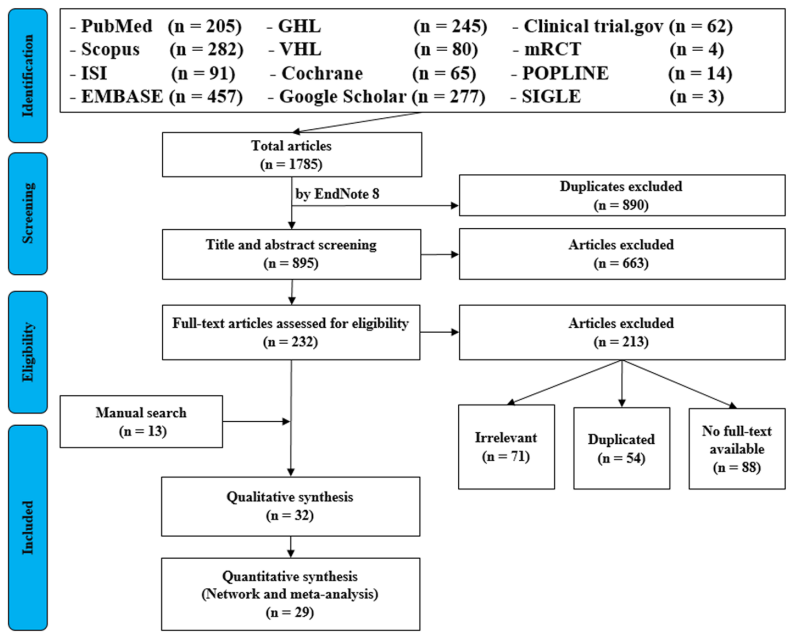
\includegraphics[width=0.8\linewidth]{sections//images/reproduced_step_by_step_guide.png}
    \caption{PRISMA flow diagram of studies' selection and screening process: Copied from \cite{tawfik_step_2019}}
    \label{fig:selection_and_screening}
\end{figure*}

\begin{table*}[t]
\centering
\small
\begin{tabular}{|c|p{0.85\textwidth}|}
\hline
\textbf{Stage} & \textbf{Purpose} \\
\hline
1 & \textbf{Framing questions for a review:} The research question is structured and explicitly formulated. \\\hline
2 & \textbf{Identifying relevant work:} A wide range of databases are searched to identify research to be included. Potential research is first identified, screened, eligibility checked, and then a decision is made on the inclusion of that research \cite{tawfik_step_2019}. \\\hline
3 & \textbf{Assessing the quality of studies:} Research is tested for quality, such as minimum research design, and subjected to higher quality assessment checks, including tests for research heterogeneity. \\\hline
4 & \textbf{Summarizing the evidence:} Data synthesis occurs with tabulation of study characteristics and quality. Statistical testing is performed at this stage. \\\hline
5 & \textbf{Interpreting the findings:} Any issues highlighted in the previous steps should be addressed. Generate recommendations guided by reference to the strength of the evidence. \\
\hline
\end{tabular}
\caption{Stages of a Systematic Review}
\label{tab:stages_of_sr}
\end{table*}

\subsubsection{Efficiency within the title and abstract Screening process}



\begin{figure*}
    \centering
    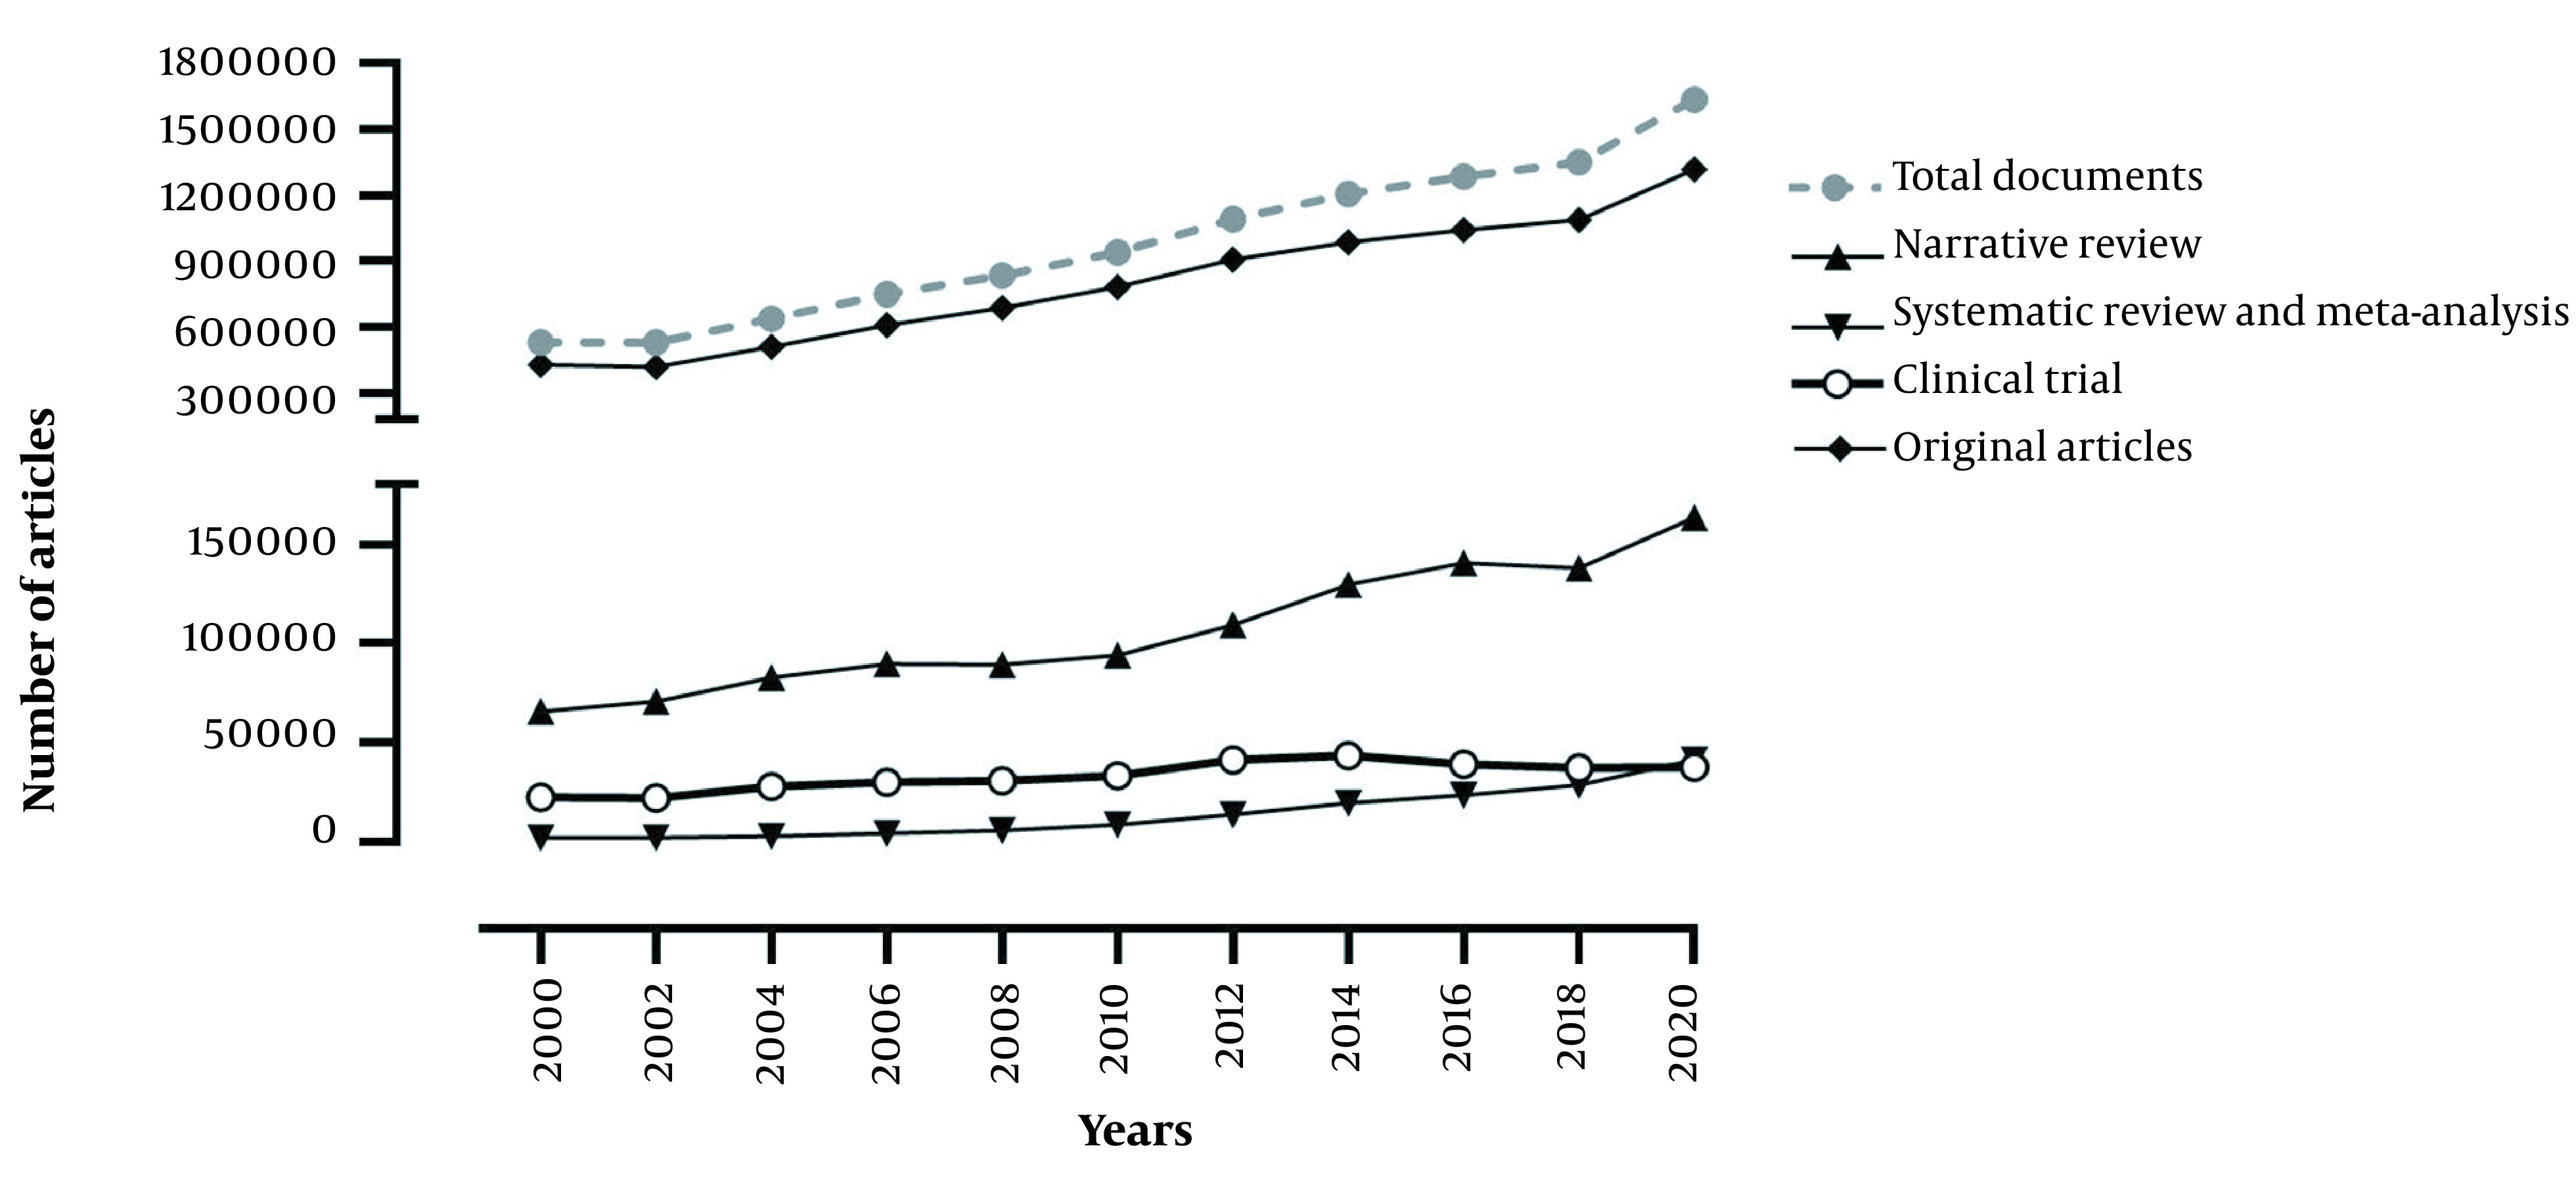
\includegraphics[width=0.8\linewidth]{sections//images/increase_in_publications.jpg}
    \caption{Increasing publications over that past two decades \cite{ghasemi_scientific_2022}}
    \label{fig:increasing_publications_over_time}
\end{figure*}

Abstract screening averages 0.13-2.88 abstracts per minute \cite{shemilt_use_2016, giummarra_evaluation_2020, felizardo_visual_2013}. Conflict resolution, which is often necessary when multiple reviewers are used (which is preferred), takes on average 5 minutes. Screening a full-text article takes 4 minutes on average \cite{shemilt_use_2016}. Given a recently released Cochrane SR on the use of preoperative statin therapy in adults undergoing cardiac surgery, we can estimate that the total time to review all the text and abstracts for this would take 7.43 hours at best and 164.64 hours at worst \cite{antunes_preoperative_nodate}. Factored into an inflation adjusted average research cost per minute (£1.598), expected costs \textbf{for just this substage alone} could be expected to be £721.97 to £15,785.68 \cite{nussbaumer-streit_resource_2021}.
\end{document}
